\documentclass[12pt]{article}
\setlength{\oddsidemargin}{0in}
\setlength{\evensidemargin}{0in}
\setlength{\textwidth}{6.5in}
\setlength{\parindent}{0in}
\setlength{\parskip}{\baselineskip}
\usepackage[all]{xy}
\usepackage[]{algorithmicx}

\usepackage{amsmath,amsfonts,amssymb}
\usepackage{graphicx}
\usepackage{fancyhdr}
\pagestyle{fancy}
\usepackage{hyperref}


\begin{document}
\lhead{{\bf CSCI 3104 \\ Problem Set 7} }
\rhead{Name: \fbox{Michael Rogers} \\ ID: \fbox{105667404} \\ {\bf Profs.\ Grochow \& Layer\\ Spring 2019, CU-Boulder}}
\renewcommand{\headrulewidth}{0.5pt}
\phantom{Test}

Quick links \ref{1} \ref{2} \ref{3a} \ref{3b} \ref{3c} \ref{4}


\vspace{-3mm}

\begin{enumerate}


\item \label{1} (10 pts) Ginerva Weasley is playing with the network given below. Help
her calculate the number of paths from node 1 to node 14.
	
Hint:\ assume a ``path'' must have at least one edge in it to be well defined,
and use dynamic programming to fill in a table that counts number of
paths from each node $j$ to 14, starting from 14 down to 1.

\[
\xymatrix{
1 \cir{} \ar[r] \ar[dr] & 2 \ar[r] \ar[dr] \ar[d] & 3 \ar[r] \ar[dr]  & 4 \ar[r] \ar[dr] \ar[d] & 5 \ar[r] \ar[dr]  & 6 \ar[d] \\
& 7 \ar[r] & 8 \ar[r] & 9 \ar[r] \ar[dr] & 10 \ar[r] \ar[dr] & 11 \ar[dr] \ar[d] \\ 
&    &    &    & 12 \ar[r] & 13 \ar[r] & 14
}
\]
\\ \\ I don't know
\pagebreak

\item \label{2} (10 pts) Ginny Weasley needs your help with her wizardly homework. She's
trying to come up with an example of a directed graph $G=(V, E)$, a start
vertex $s \in V$ and a set of tree edges $E_{T} \subseteq E$ such that
for each vertex $v \in V$, the unique path in the graph $(V,E_{T})$
from $s$ to $v$ is a shortest path in $G$, yet the set of edges $E_{T}$
cannot be produced by running a depth-first search on $G$, no matter
how the vertices are ordered in each adjacency list. Include an
explanation of why your example satisfies the requirements.\\
\\ \\ I don't know
\pagebreak


\item Prof.\ Dumbledore needs your help to compute the in- and out-degrees of all vertices in a directed multigraph $G$. However, he is not sure how to represent the graph so that the calculation is most efficient. For each of the three possible representations, express your answers in asymptotic notation (the only notation Dumbledore understands), in terms of $V$ and $E$, and justify your claim.
\begin{enumerate}
\item \label{3a} (5 pts) An {\em adjacency matrix} representation. Assume the size of the matrix is known.
\\ \\ I don't know
\pagebreak
\item \label{3b} (5 pts) An {\em edge list} representation. Assume vertices have arbitrary labels.
\\ \\ I don't know
\pagebreak
\item \label{3c} (5 pts) An {\em adjacency list} representation. Assume the vector's length is known.
\\ \\ I don't know
\pagebreak
\end{enumerate}


\item \label{4} (25 pts) Deep in the heart of the Hogwarts School of Witchcraft and
Wizardry, there lies a magical grey parrot that demands that any challenger
efficiently convert directed multigraphs into directed \emph{simple}
graphs. If the wizard can correctly solve a series of arbitrary
instances of this problem, the parrot will unlock a secret passageway. 

% ----- FIGURE 1 : adjacency_list.eps -----
\begin{figure}[h!]
\begin{center}
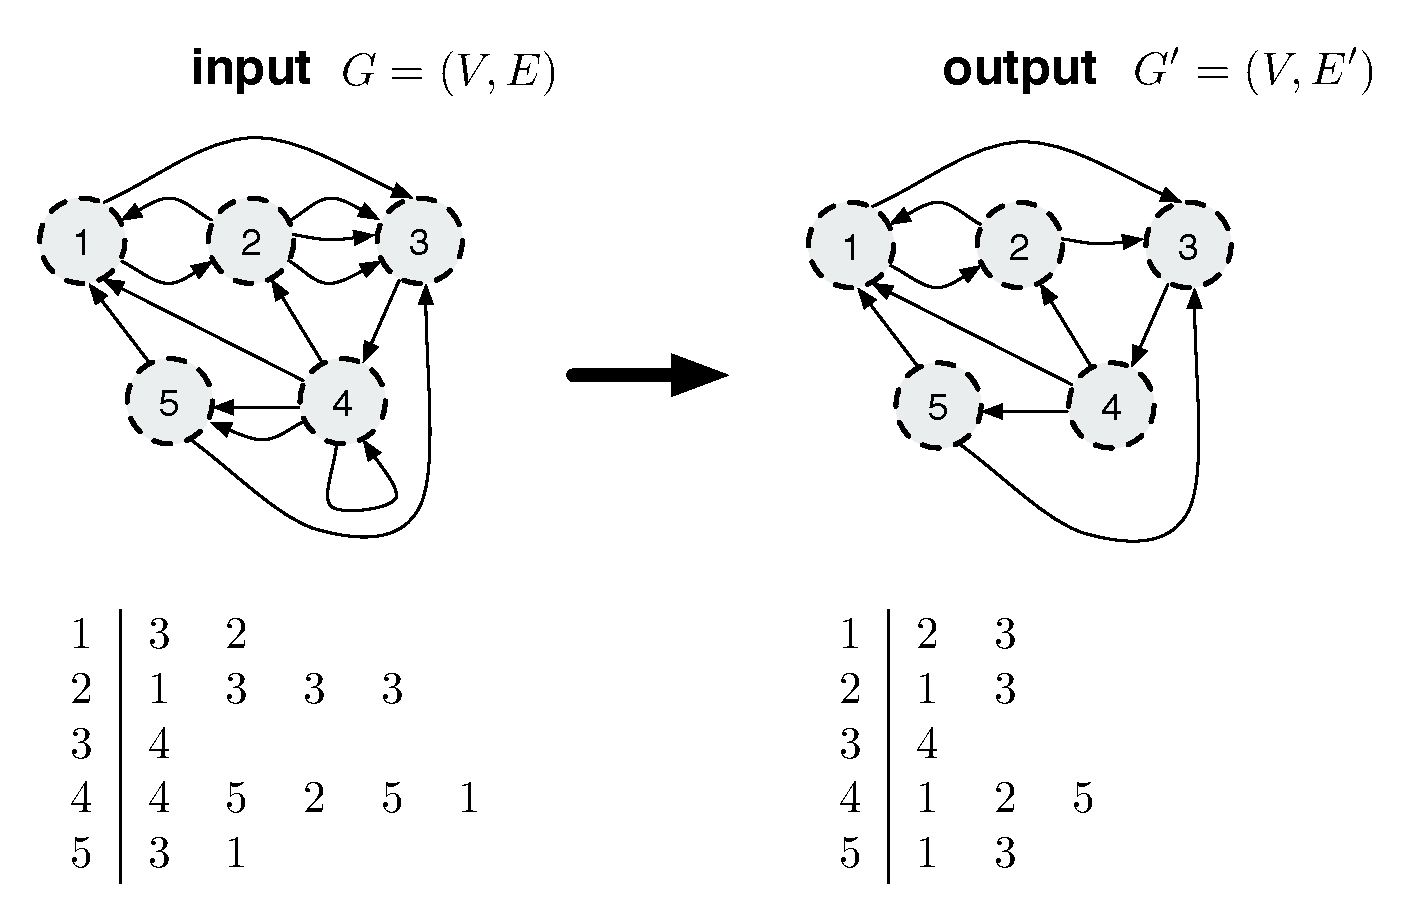
\includegraphics[scale=0.5]{adjacency_list.eps} \\
An example of transforming $G\to G'$
\end{center}
\label{fig:adjlist}
\end{figure}
% ----------
	
Let $G=(E,V)$ denote a directed multigraph. A directed simple graph is a
$G'=(V,E')$, such that $E'$ is derived from the edges in $E$ so that (i)~every
directed multi-edge, e.g., $\{(u,v),(u,v)\}$ or even simply $\{(u,v)\}$, has
been replaced by a single directed edge $\{(u,v)\}$ and (ii)~all self-loops
$(u,u)$ have been removed.\\
\pagebreak

Describe and analyze an algorithm (explain how it works, give pseudocode if
necessary, derive its running time and space usage, and prove its correctness)
that takes \mbox{$O(V+E)$} time and space to convert $G$ into $G'$, and thereby
will solve any of the parrot's questions. Assume both $G$ and $G'$ are stored
as adjacency lists.
	
Hermione's hints: Don't assume adjacencies {\tt Adj[u]} are ordered in any
particular way, and remember that you can add edges to the list and then remove
ones you don't need.\\
\\ \\ I don't know
\pagebreak

\end{enumerate}
\end{document}
